%%
%% licence       kaneton licence
%%
%% project       kaneton
%%
%% file          /home/buckman/kaneton/view/lectures/kernels/tp-k0/tp-k0.tex
%%
%% created       matthieu bucchianeri   [wed jan 24 14:46:51 2007]
%% updated       matthieu bucchianeri   [wed jan 24 15:10:21 2007]
%%

%
% template
%

%
% ---------- header -----------------------------------------------------------
%
% project       kaneton
%
% license       kaneton
%
% file          /home/mycure/kaneton/view/template/paper.tex
%
% created       julien quintard   [wed may 16 18:17:37 2007]
% updated       julien quintard   [fri oct  5 07:00:45 2007]
%

%
% class
%

\documentclass[10pt,a4wide]{article}

%
% packages
%

\usepackage[english]{babel}
\usepackage[T1]{fontenc}
\usepackage{a4wide}
\usepackage{fancyheadings}
\usepackage{multicol}
\usepackage{indentfirst}
\usepackage{graphicx}
\usepackage{color}
\usepackage{xcolor}
\usepackage{verbatim}
\usepackage{aeguill}

\pagestyle{fancy}

\setlength{\footrulewidth}{0.3pt}
\setlength{\parindent}{0.3cm}
\setlength{\parskip}{2ex plus 0.5ex minus 0.2ex}

%
% logos
%

\newcommand{\logos}
  {
    \begin{center}
      
\includegraphics[scale=0.8]{\path/logo/kaneton.pdf}
    \end{center}
  }

%
% prototype
%

\newcommand\prototype[2]{
  \begin{tabular}{p{0.2cm}p{13.8cm}}
  & #1
  \end{tabular}

  \begin{tabular}{p{1cm}p{13cm}}
  & #2
  \end{tabular}}

%
% verbatim stuff
%

\definecolor{verbatimcolor}{rgb}{0.00,0.40,0.00}

\makeatletter

\renewcommand{\verbatim@font}
  {\ttfamily\footnotesize\selectfont}

\def\verbatim@processline{
  {\color{verbatimcolor}\the\verbatim@line}\par
}

\makeatother

%
% header
%

\rhead{}
\rfoot{\scriptsize{The kaneton microkernel project}}

\date{\scriptsize{\today}}

\usepackage{pdfpages}

%
% header
%

\lhead{\scriptsize{k0}}

%
% title
%

\title{kaneton K0\\Bootstrap}

%
% authors
%

\author{\small{Matthieu Bucchianeri} and
        \small{Renaud Voltz}}

%
% document
%

\begin{document}

\maketitle

\vspace{5mm}

\begin{tabular}{p{7cm}l}
Delivery date: & Sunday, 28th \\
               & 11:42 pm \\
Assistants : & Matthieu Bucchianeri - \small{chichelover@epita.fr} \\
             & Renaud Voltz - \small{voltz\_r@epita.fr} \\
Dedicated googlegroup: & kaneton-students \\
Programming languages: & Assembly, C \\
Architecture: & Intel 32-bit \\
Students per group: & 1
\end{tabular}

\subsection*{Introduction}

\newpage

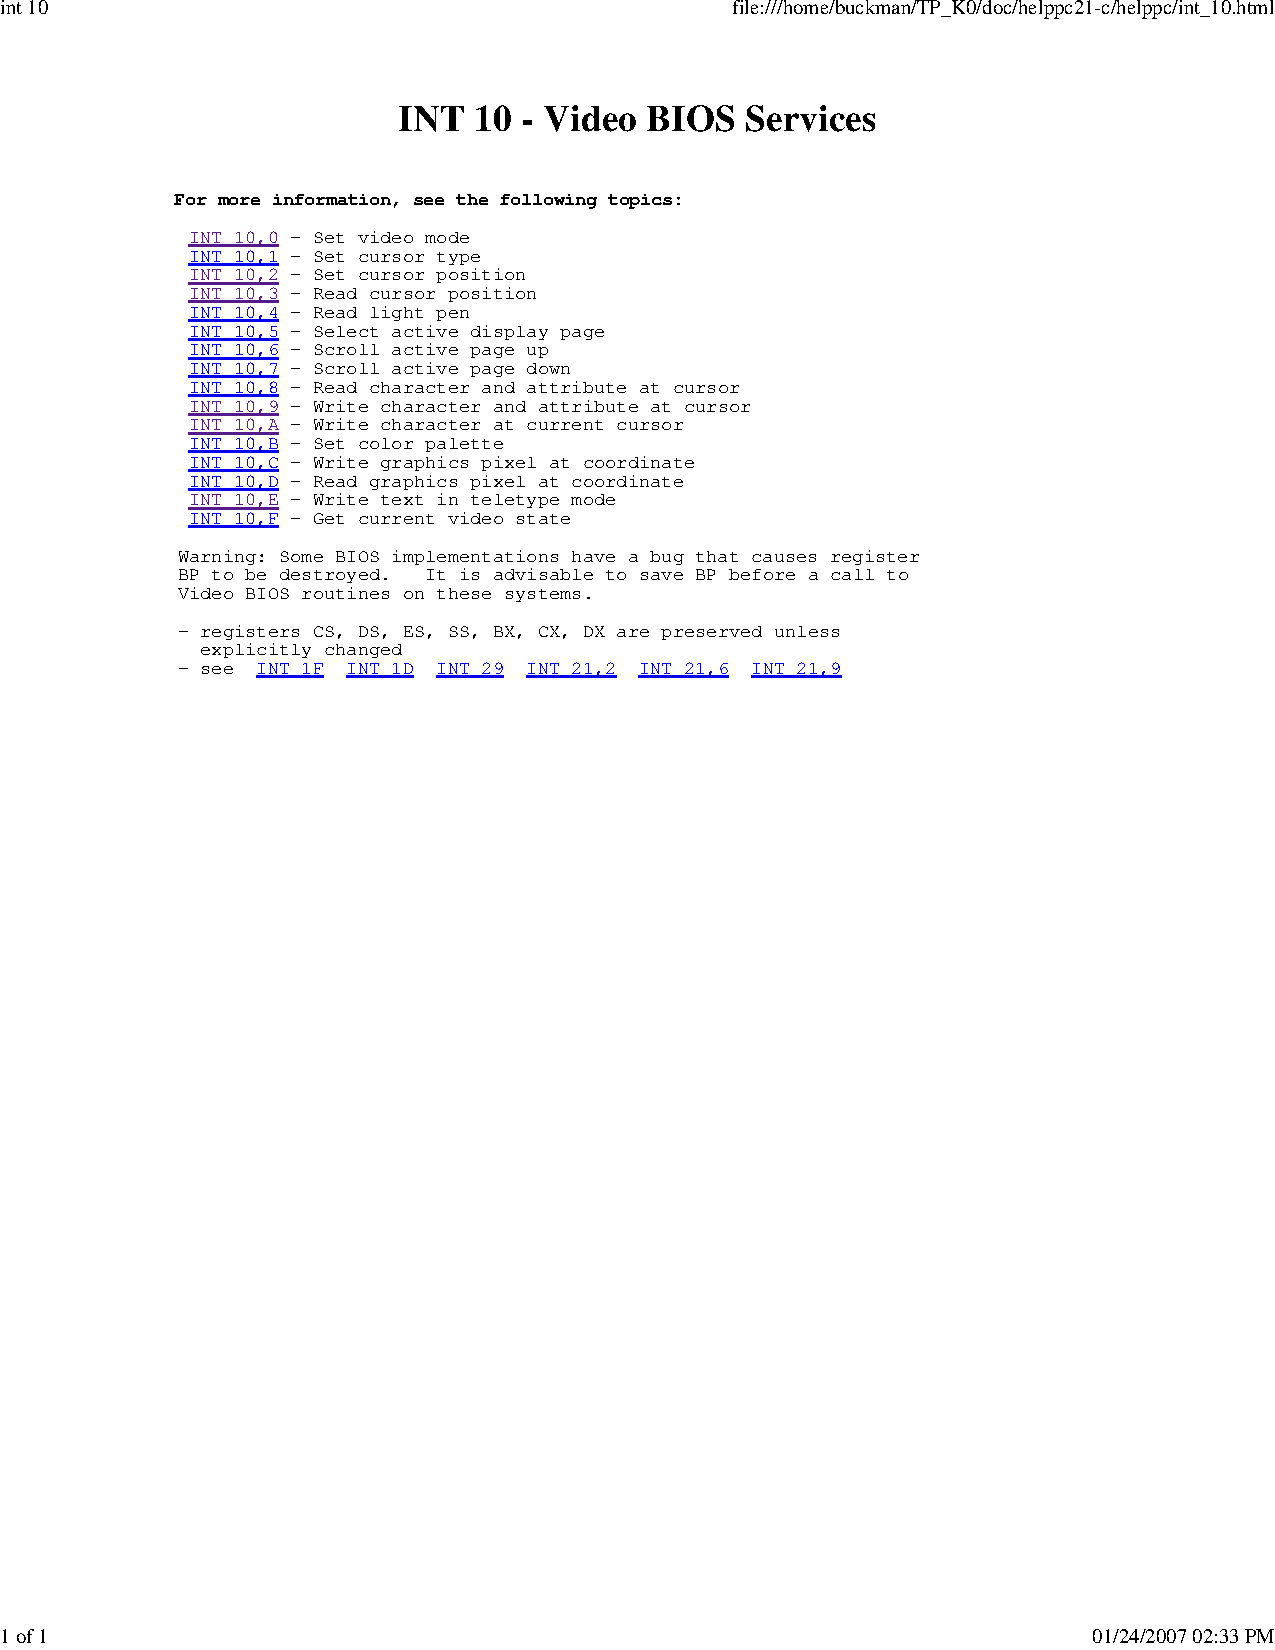
\includepdf[pages=-]{int10}
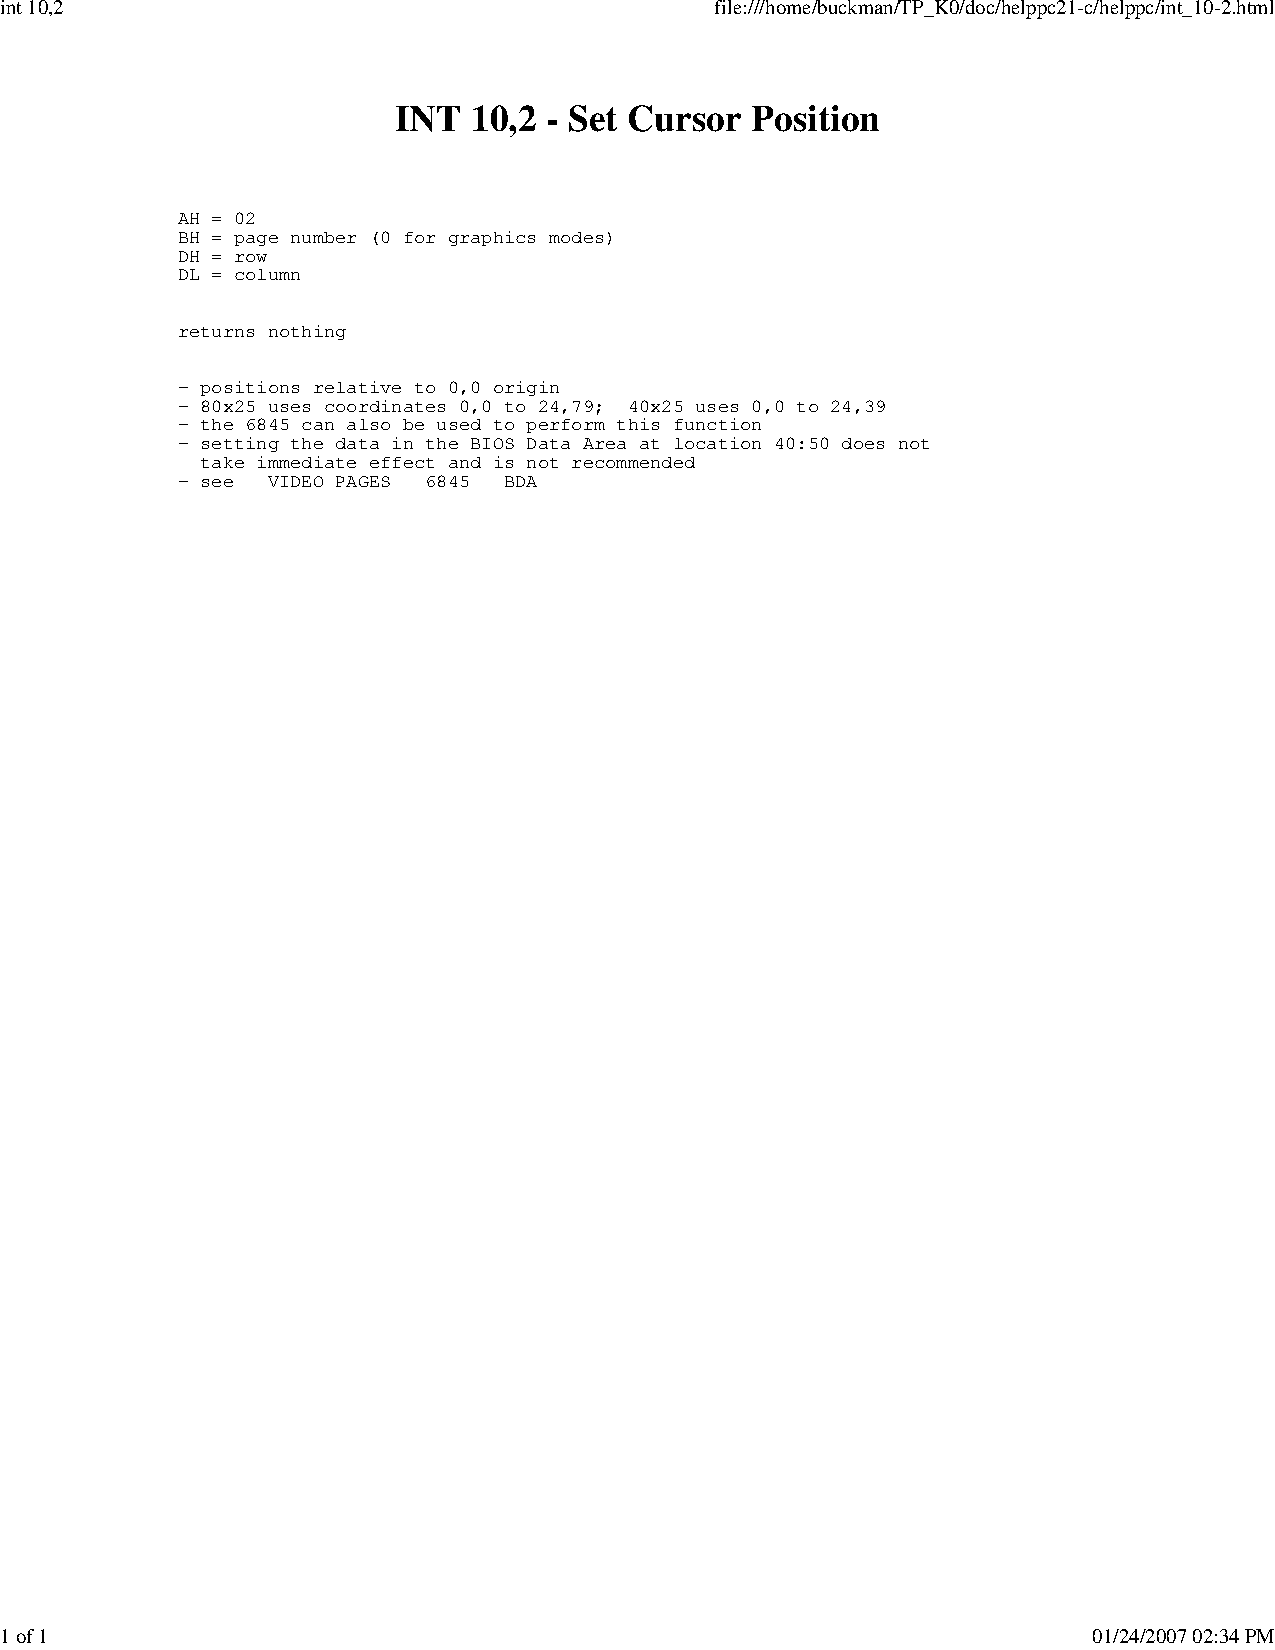
\includepdf[pages=-]{int10_2}
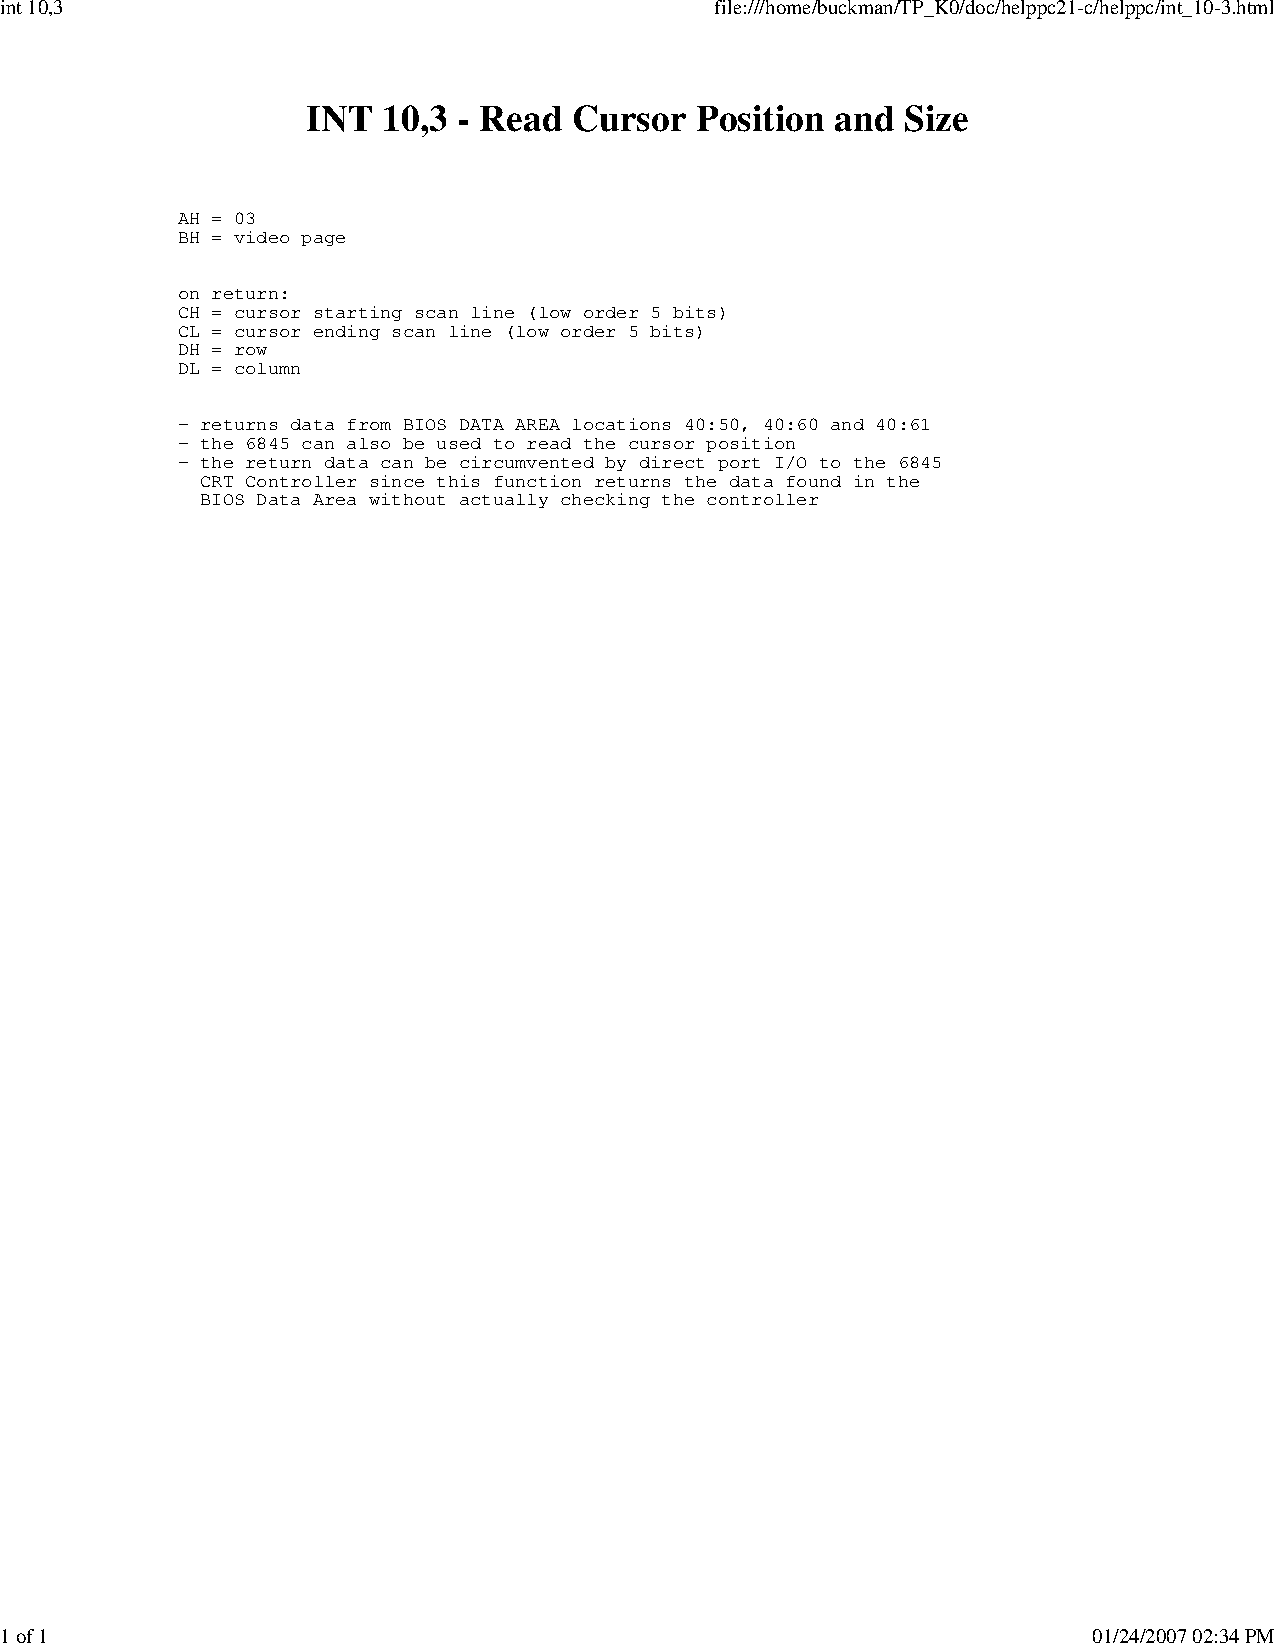
\includepdf[pages=-]{int10_3}
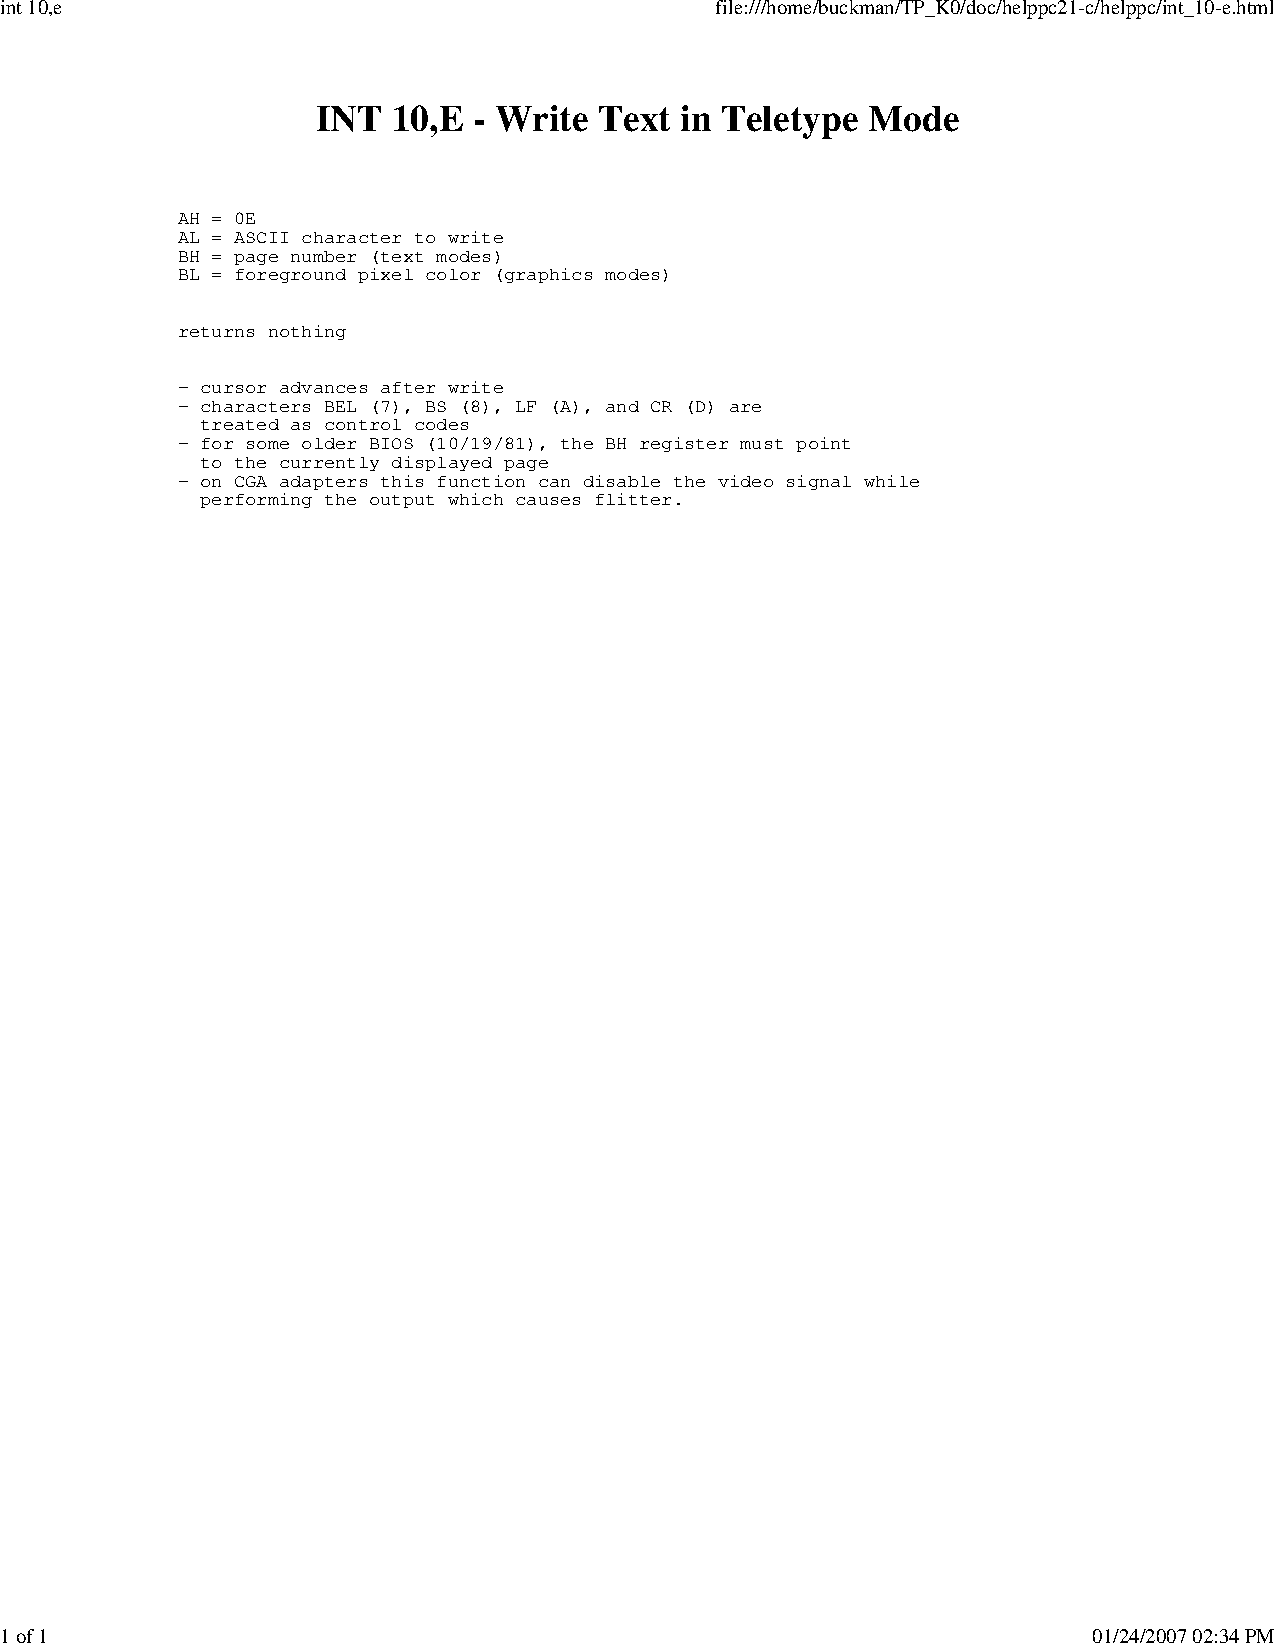
\includepdf[pages=-]{int10_e}

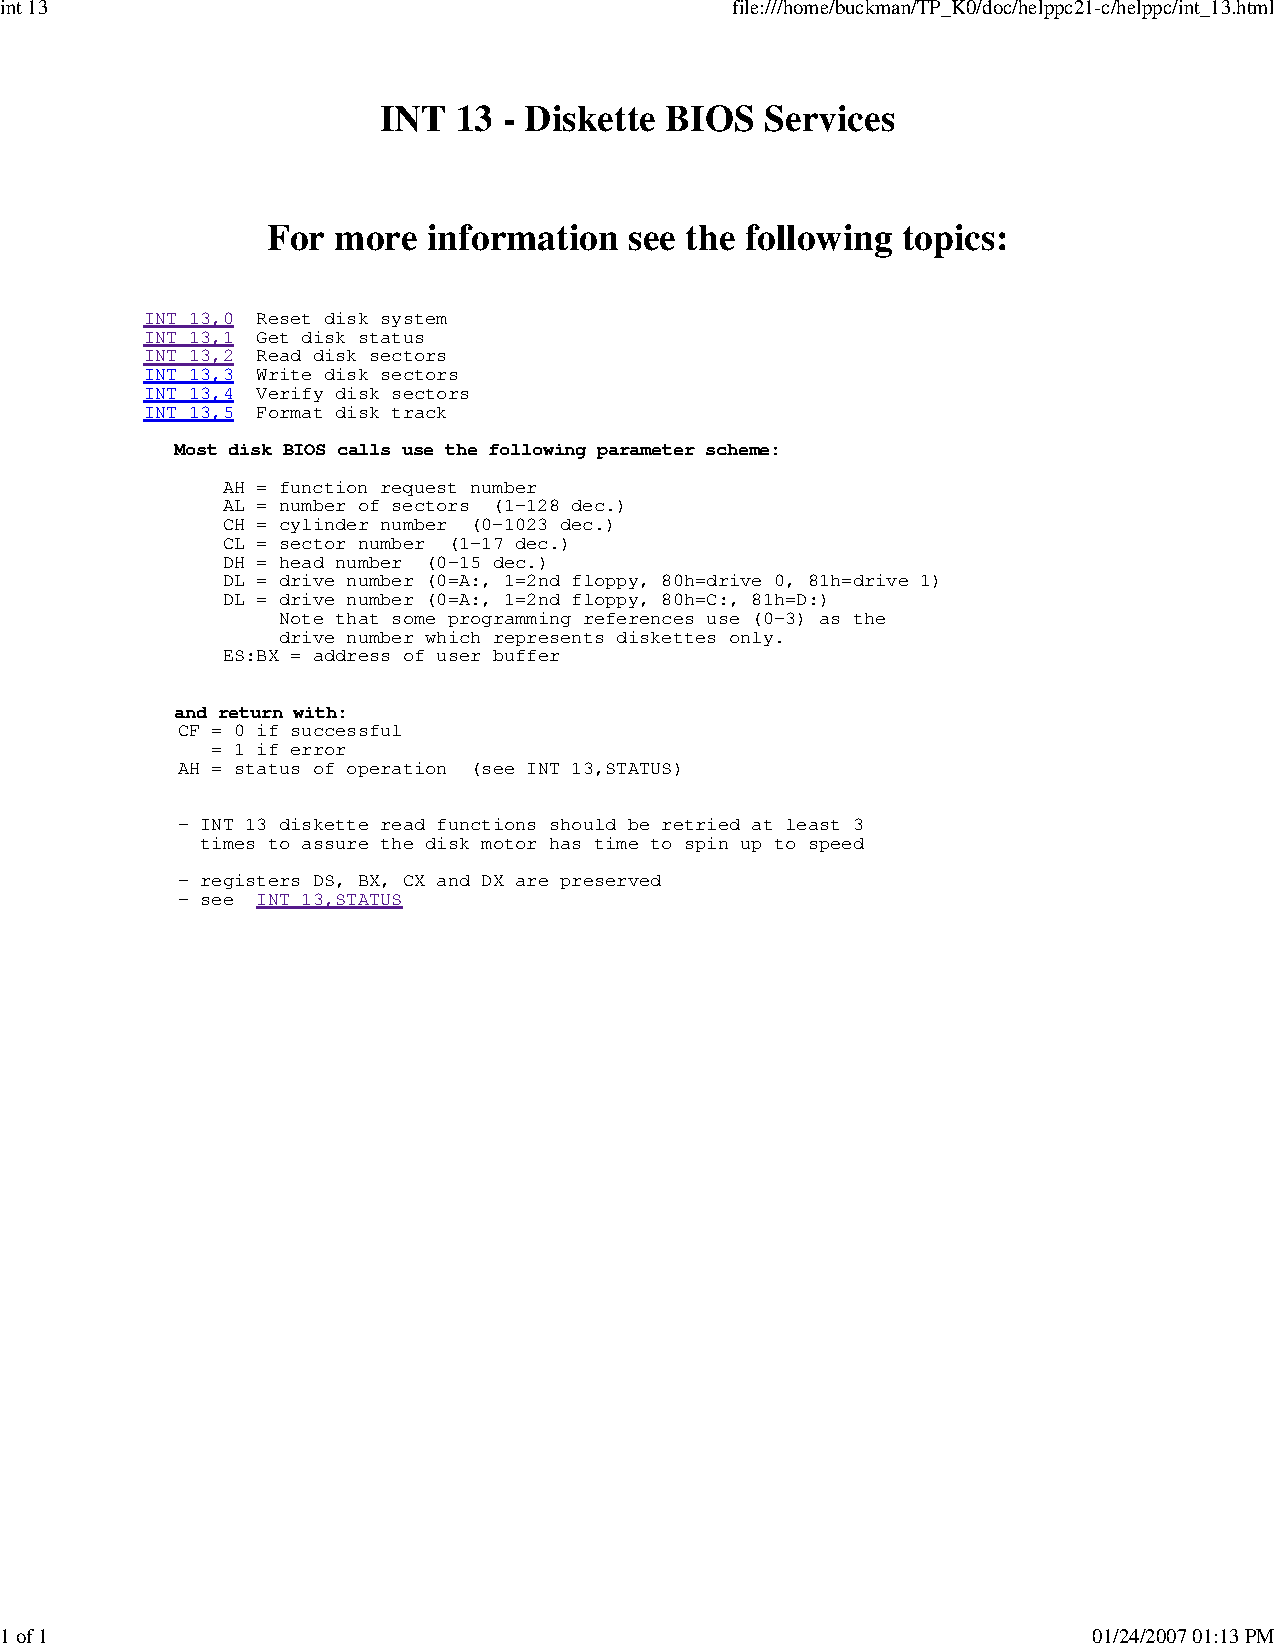
\includepdf[pages=-]{int13}
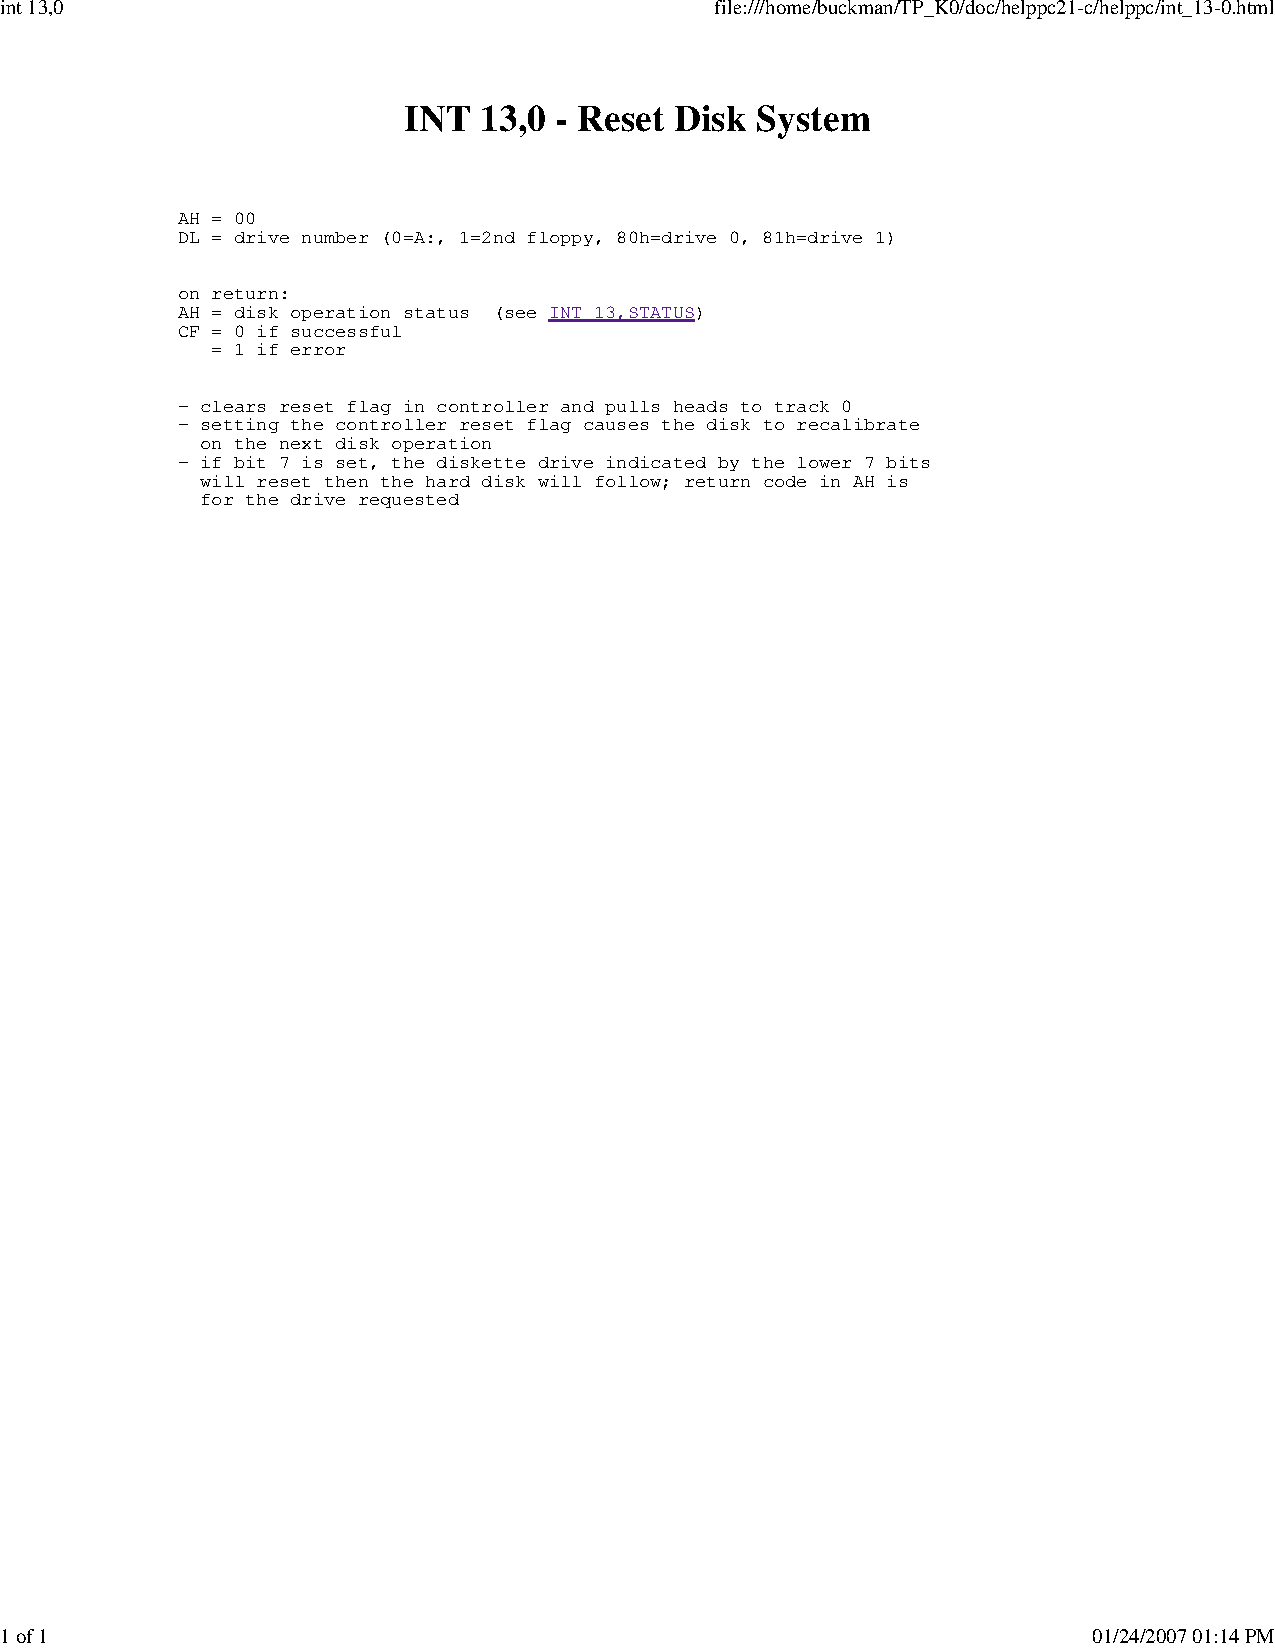
\includepdf[pages=-]{int13_0}
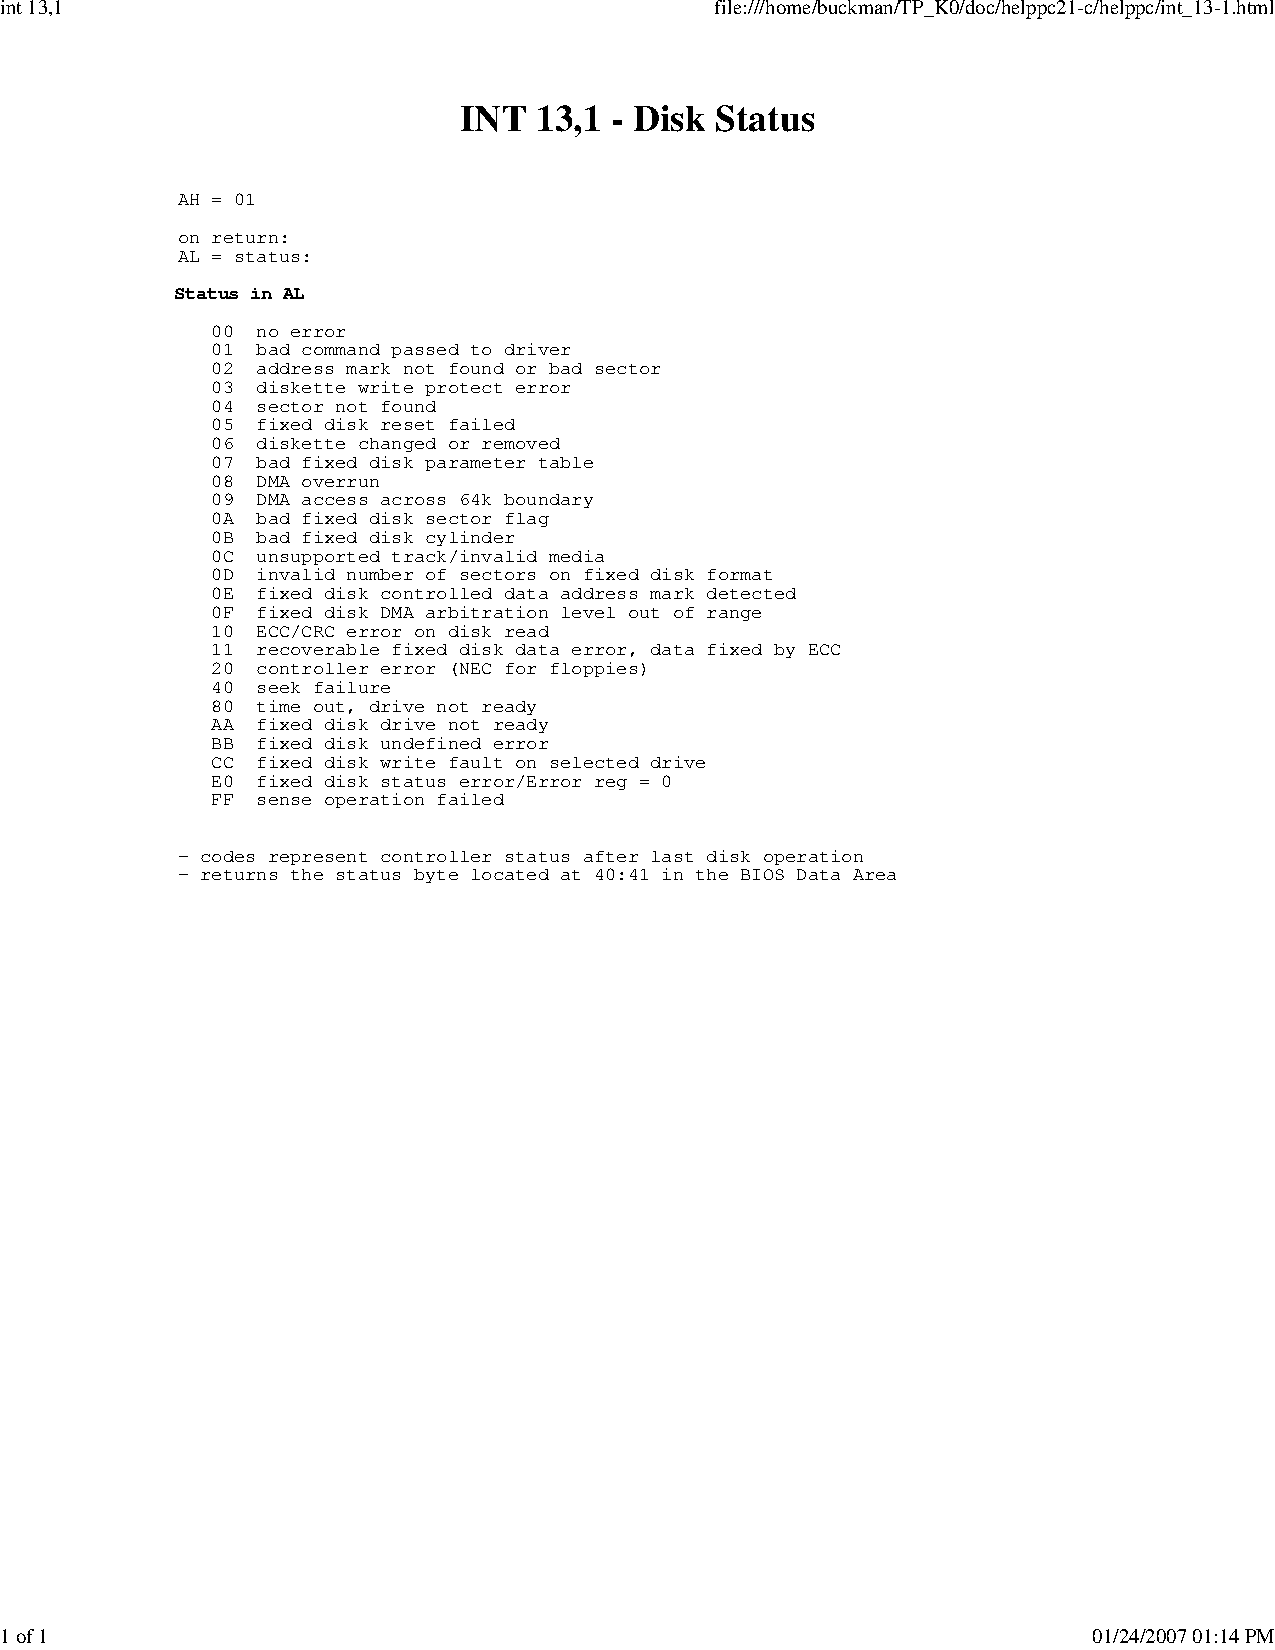
\includepdf[pages=-]{int13_1}
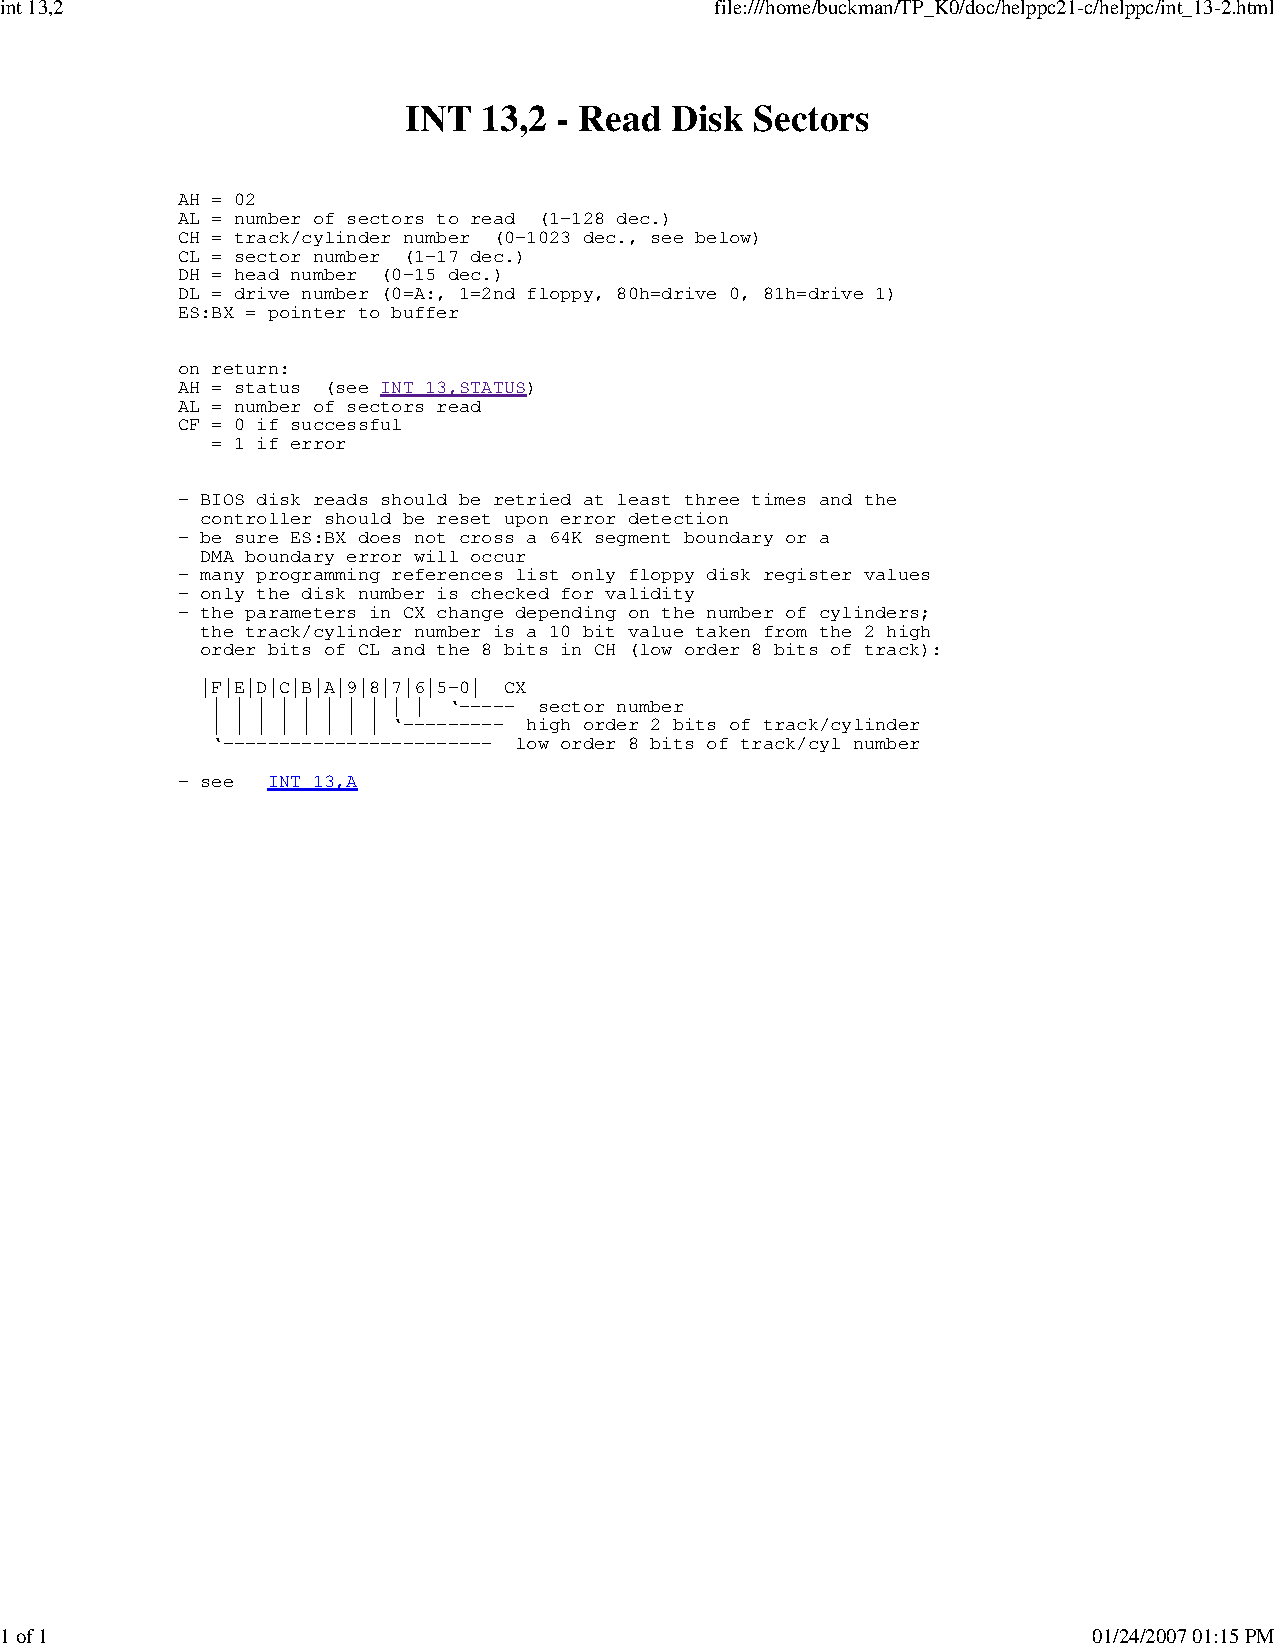
\includepdf[pages=-]{int13_2}

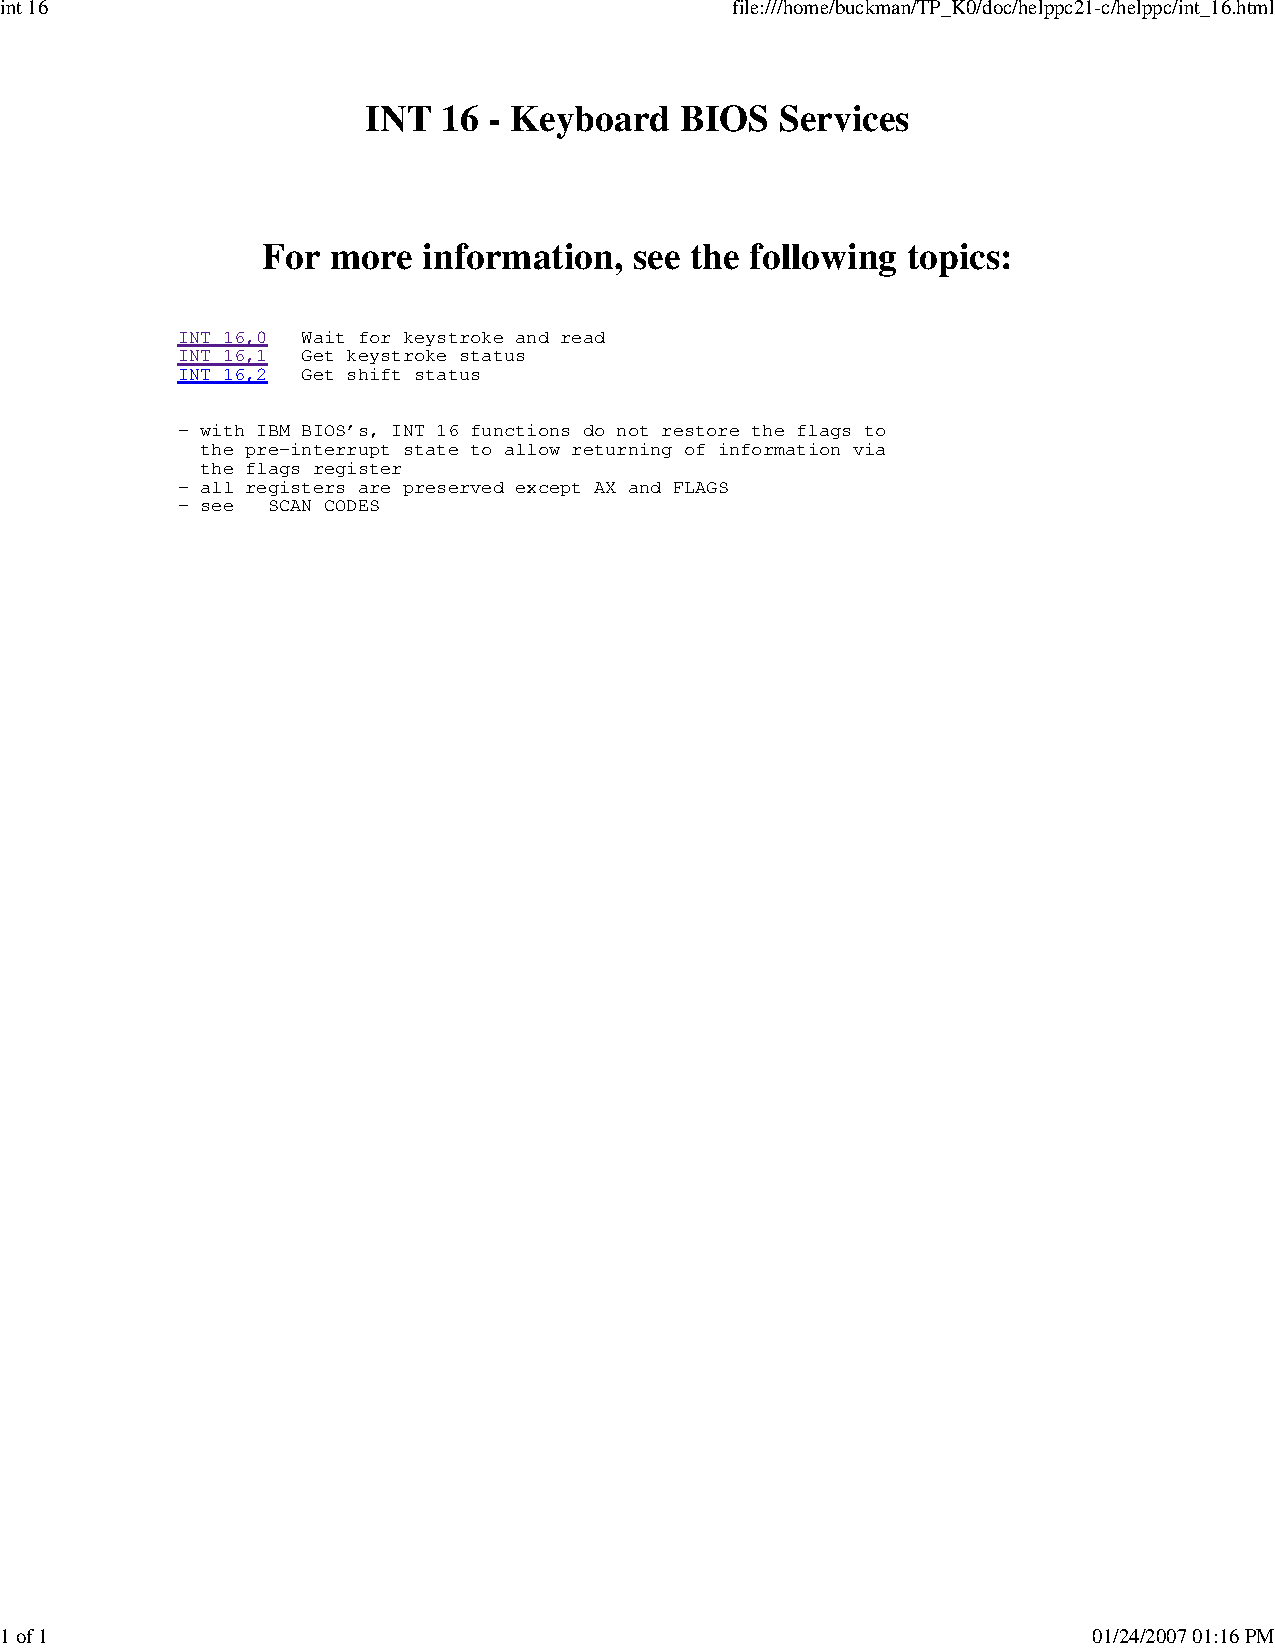
\includepdf[pages=-]{int16}
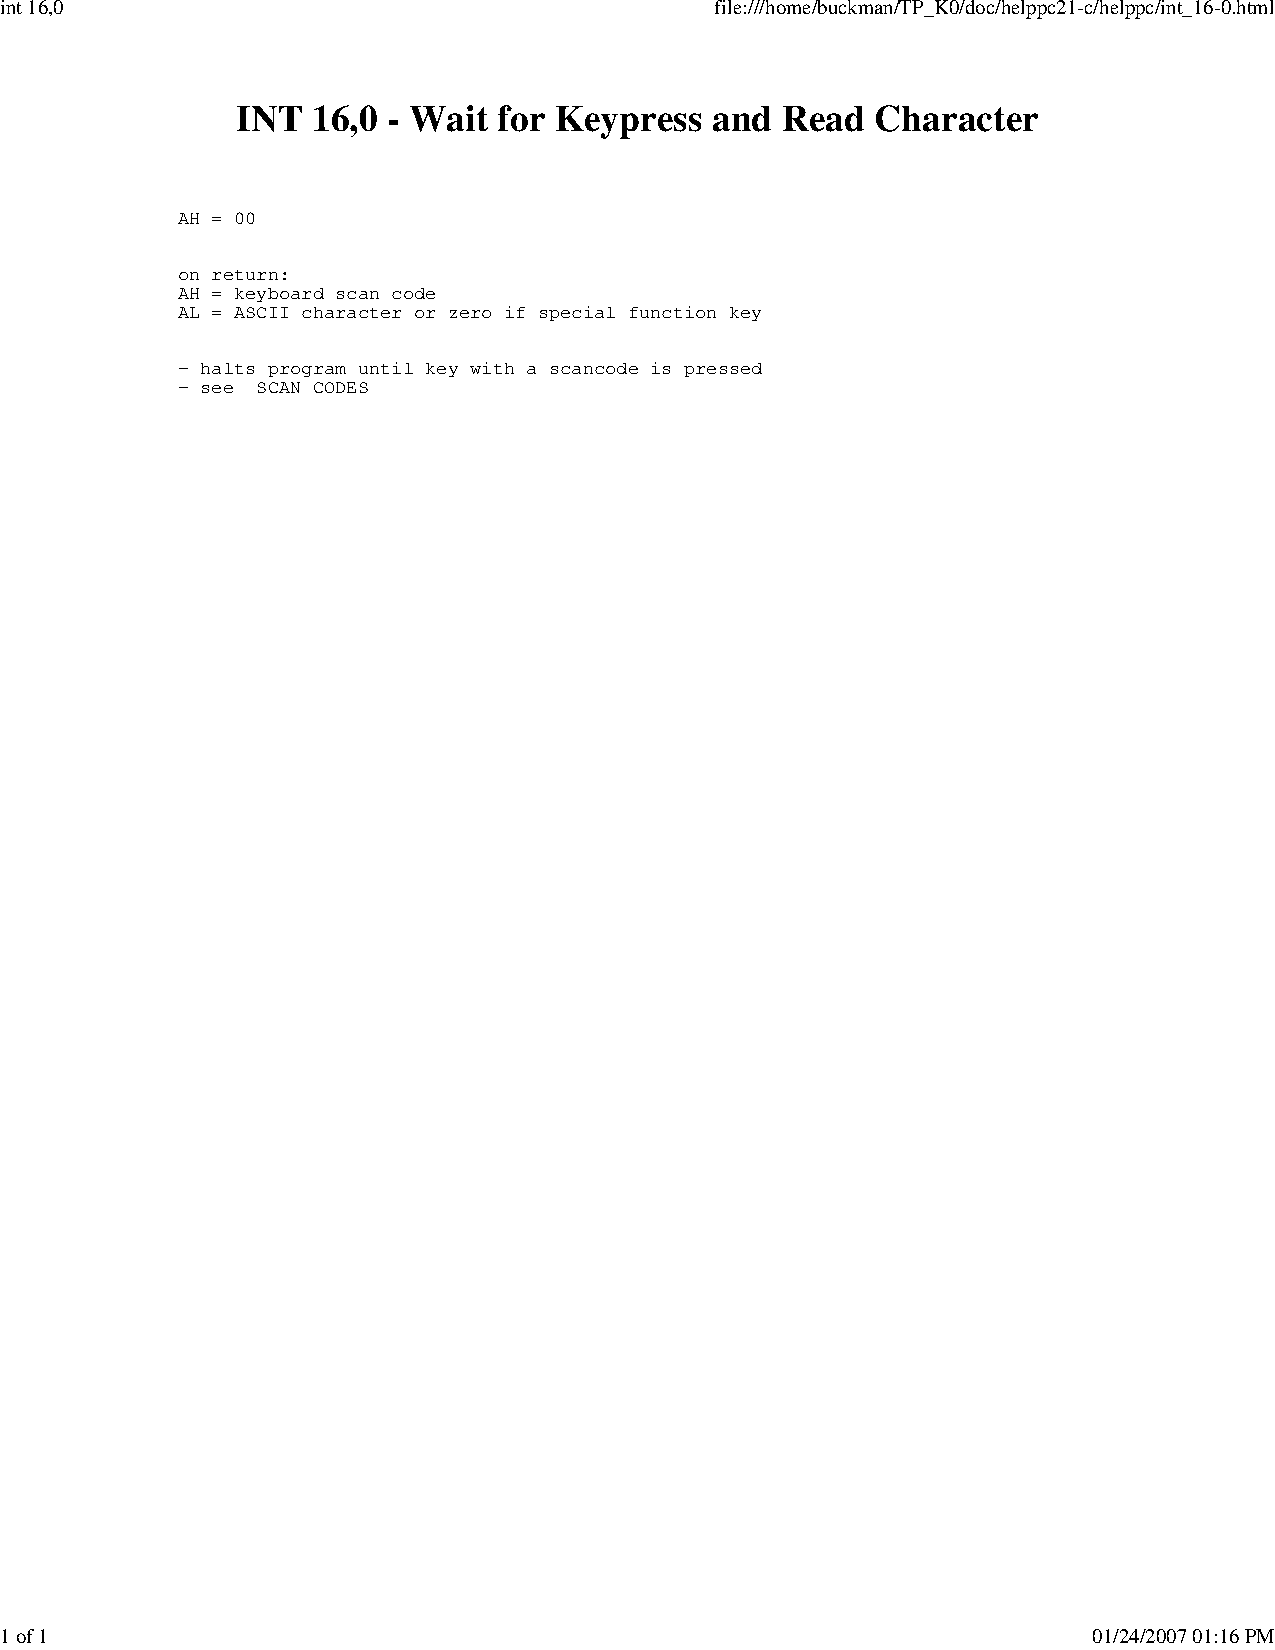
\includepdf[pages=-]{int16_0}
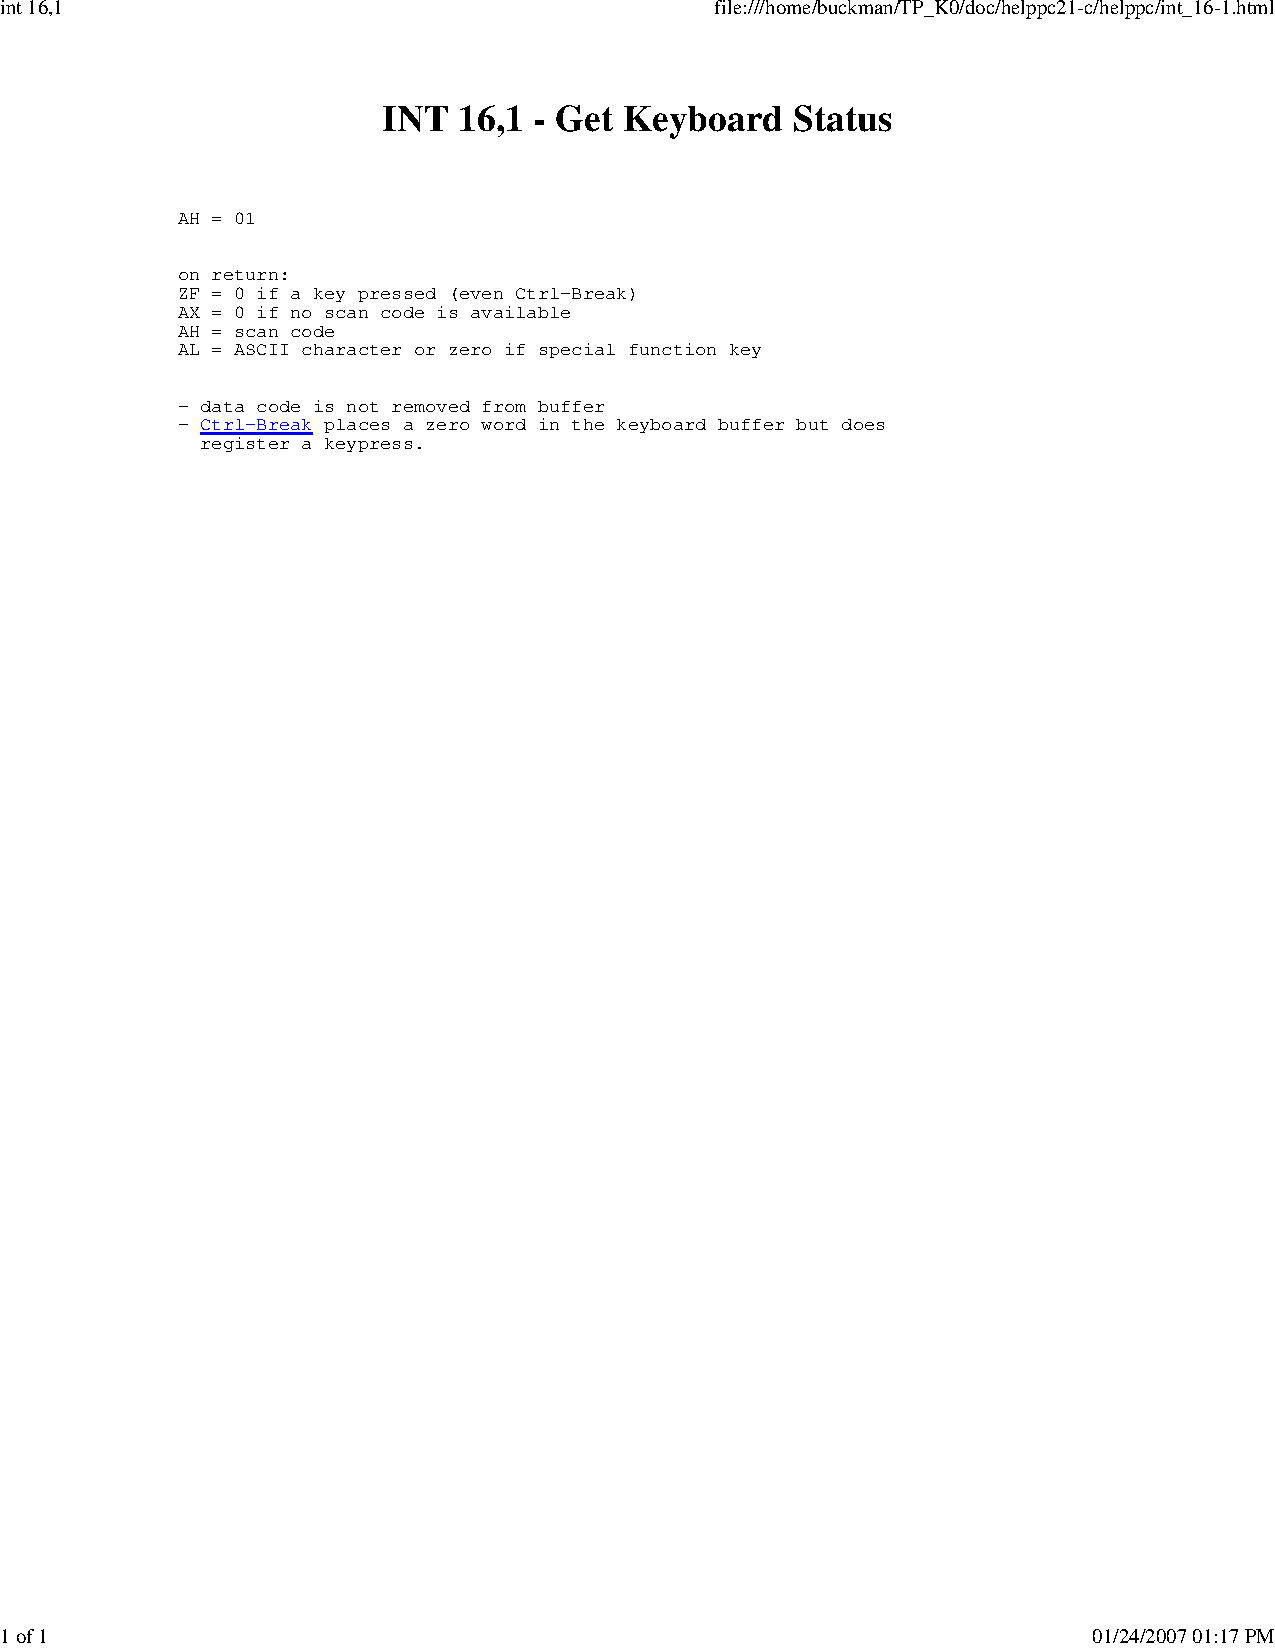
\includepdf[pages=-]{int16_1}
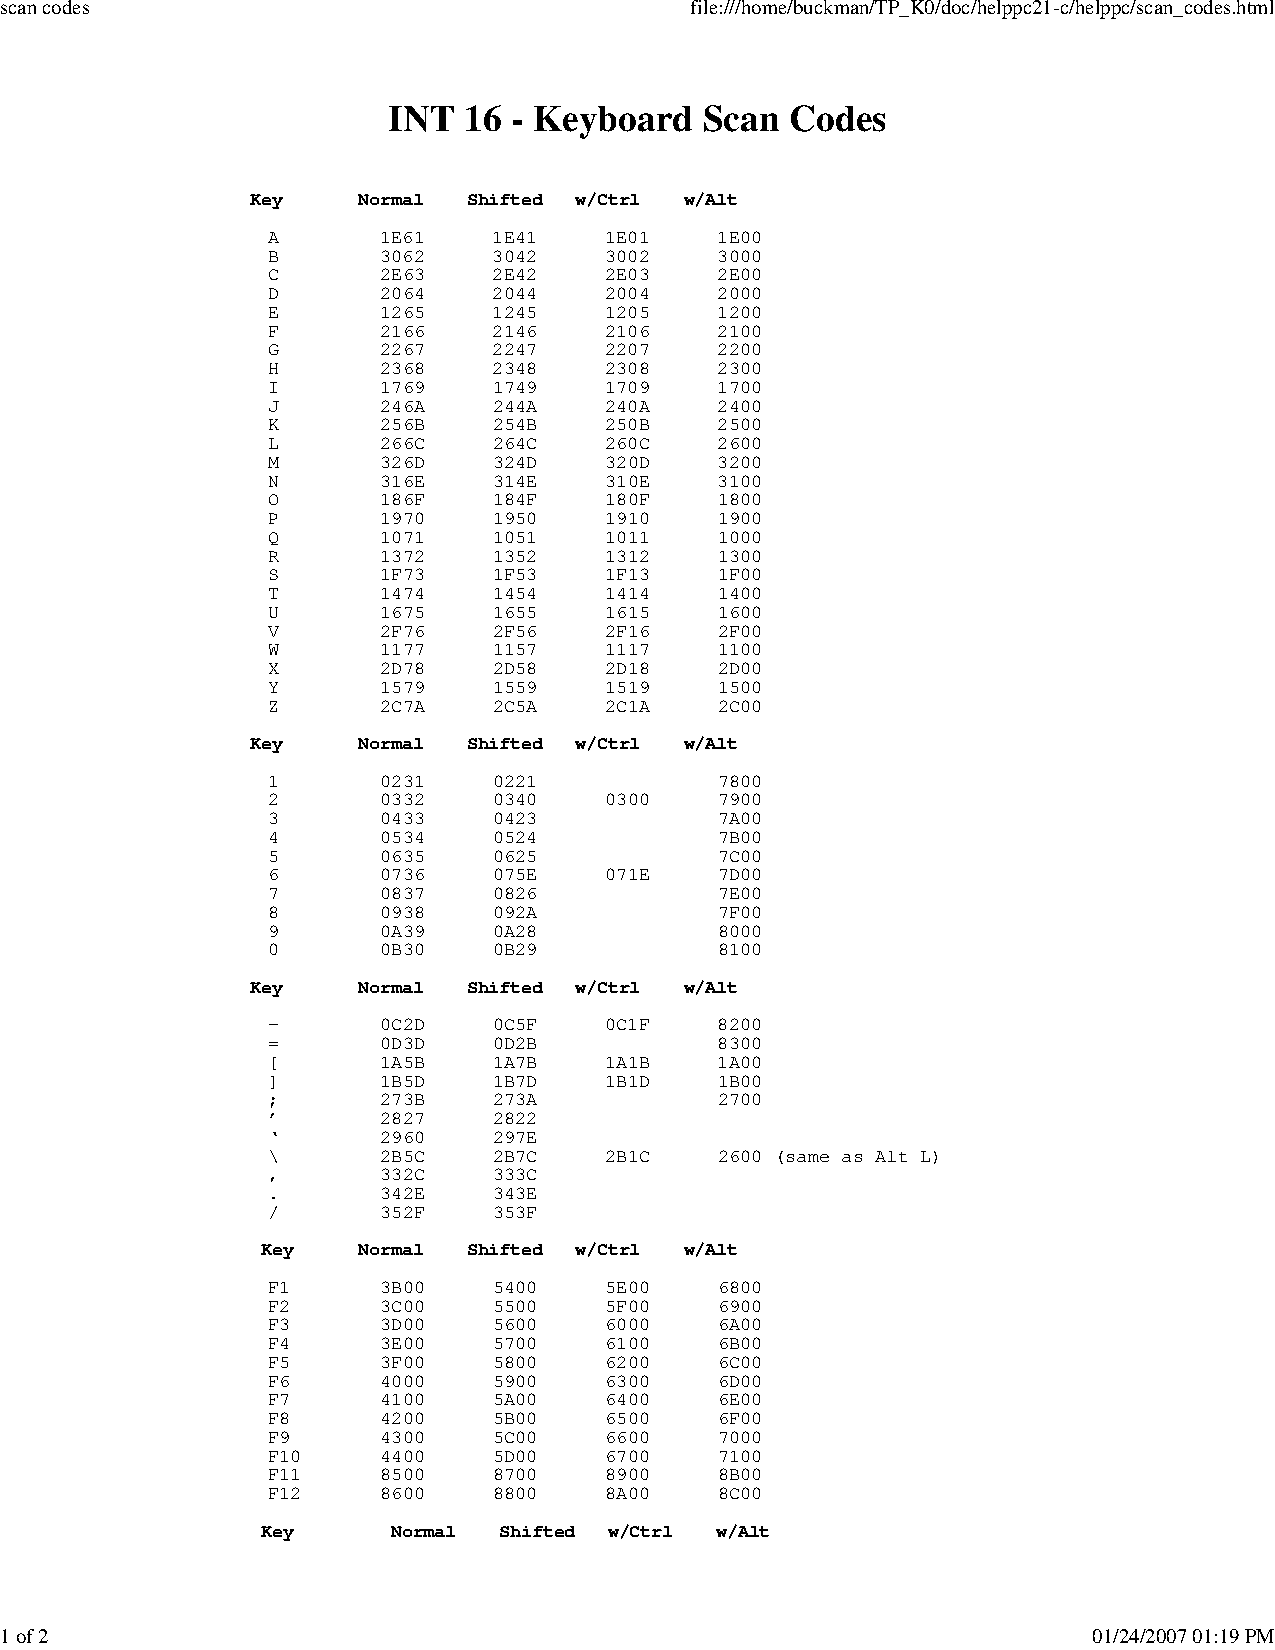
\includepdf[pages=-]{int16_scancodes}

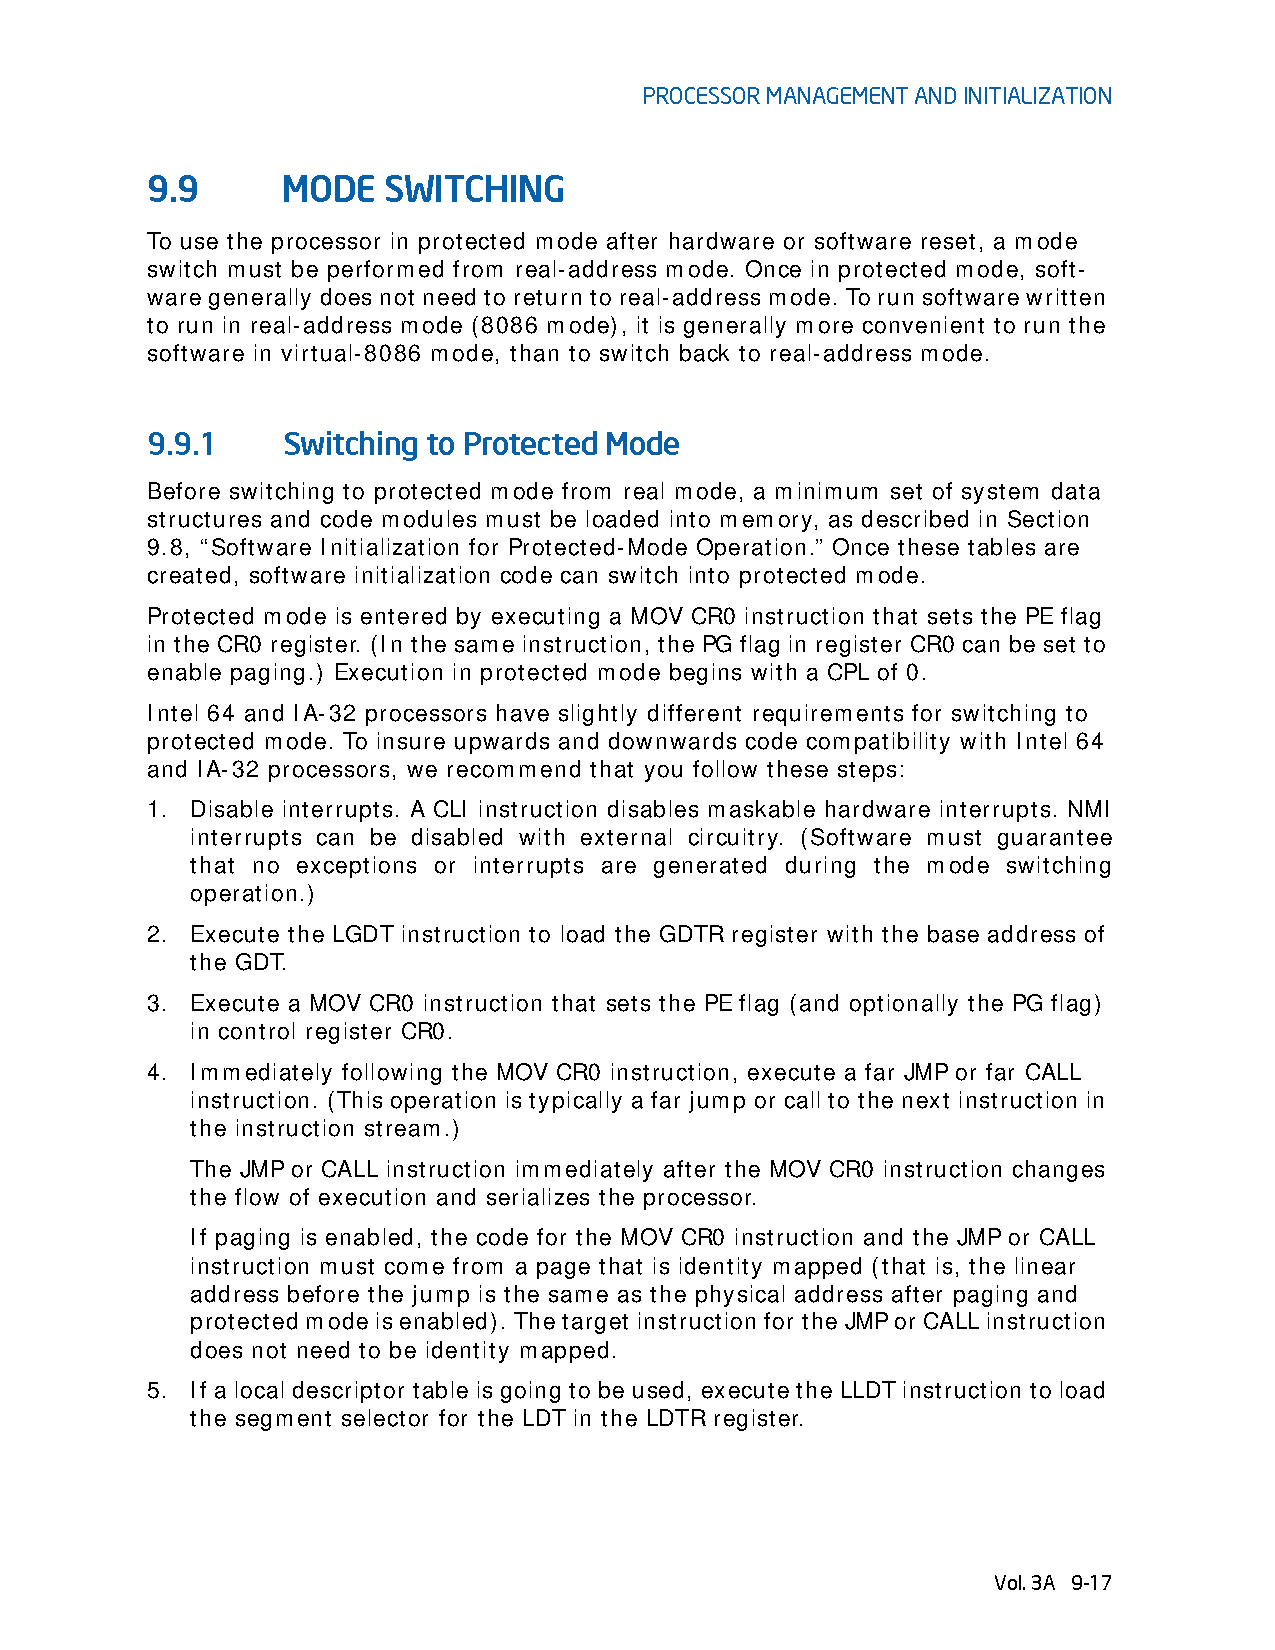
\includepdf[pages=-]{mode_switch}

\end{document}
